\documentclass{article}

\usepackage{noweb}
\noweboptions{smallcode,longchunks}

\usepackage[a4paper,margin=1in]{geometry}

\usepackage{colortbl}
\usepackage[colorlinks=true]{hyperref}
\usepackage{graphicx}

% Define a handy paragraph opener
\newcommand{\hi}[1]{\noindent {\bf #1}}

% Remove noweb page break penalty
\def\nwendcode{\endtrivlist \endgroup}
\let\nwdocspar=\par

\title{Jargo Simulation Controller\footnote{\url{https://github.com/jargors/Simulation-Controller}}}
\author{James J. Pan\\
  \small{\href{mailto:jamesjpan@outlook.com}{jamesjpan@outlook.com}}
}

\begin{document}
\maketitle
\pagestyle{noweb}

\tableofcontents

\section{Introduction}
\label{sec:introduction}
The simulation controller is designed to be the sole means of an evaluation
program for controlling Jargo's simulation environment. The controller is
responsible for advancing the simulation world time, ``pushing'' server
locations and new requests to the client, perturbing server routes stored in
the data layer to mimic real-world stochastic traffic and vehicle processes,
and reporting evaluation metrics to the evaluation program.  The simulation
controller is developed using the
Noweb\footnote{\url{https://www.cs.tufts.edu/~nr/noweb/}} literate
programming\footnote{\url{http://literateprogramming.com/}} tool.  This file
({\tt{}src/SimulationController.nw}) is the source for both the documentation
({\tt{}doc/SimulationController.tex}) and the Java code
({\tt{}SimulationController.java})\footnote{See the {\tt{}Makefile} for build
details.}.

\begin{figure}[h]
\centering
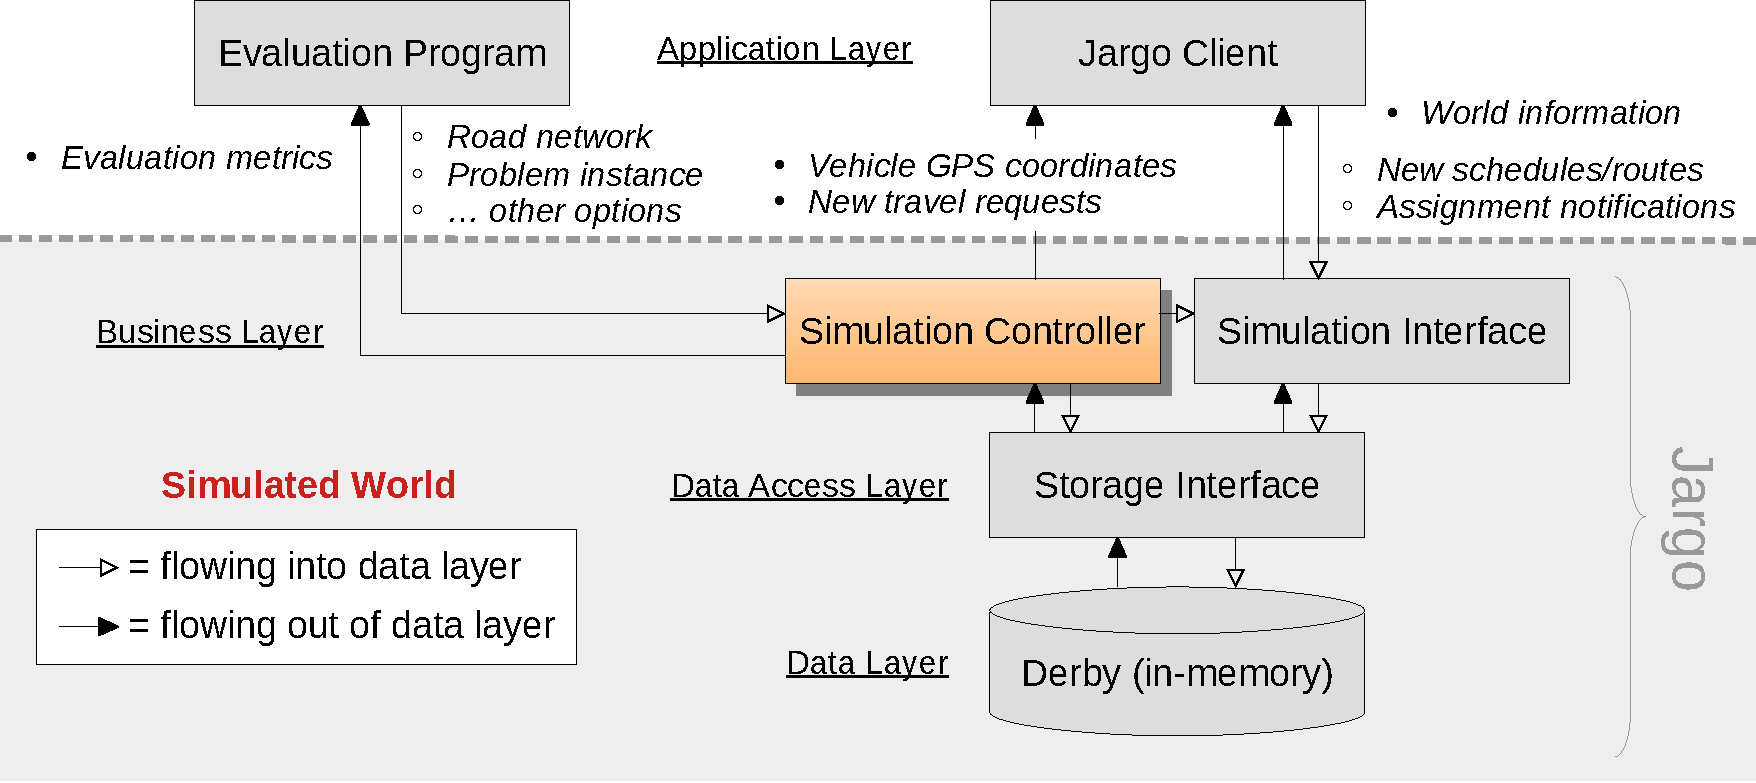
\includegraphics[width=150mm]{src/fig/controller-fig}
\caption{Controller within the Jargo stack.}
\label{fig:controller}
\end{figure}

\section{Implementation Overview}
\nwfilename{src/SimulationController.nw}\nwbegincode{1}\sublabel{NW3Xlx2m-wPE4K-1}\nwmargintag{{\nwtagstyle{}\subpageref{NW3Xlx2m-wPE4K-1}}}\moddef{SimulationController.java~{\nwtagstyle{}\subpageref{NW3Xlx2m-wPE4K-1}}}\endmoddef\nwnotused{SimulationController.java}
  \LA{}SimulationController.java preamble~{\nwtagstyle{}\subpageref{NW3Xlx2m-2MWOaE-1}}\RA{}
  \LA{}\code{}SimulationController\edoc{} definition~{\nwtagstyle{}\subpageref{NW3Xlx2m-2ZG2N7-1}}\RA{}
\nwendcode{}\nwbegindocs{2}\nwdocspar

\subsection{Preamble}
\nwenddocs{}\nwbegincode{3}\sublabel{NW3Xlx2m-2MWOaE-1}\nwmargintag{{\nwtagstyle{}\subpageref{NW3Xlx2m-2MWOaE-1}}}\moddef{SimulationController.java preamble~{\nwtagstyle{}\subpageref{NW3Xlx2m-2MWOaE-1}}}\endmoddef\nwalsodefined{\\{NW3Xlx2m-2MWOaE-2}\\{NW3Xlx2m-2MWOaE-3}}\nwused{\\{NW3Xlx2m-wPE4K-1}}
package com.github.jargors;
\nwendcode{}\nwbegindocs{4}\nwdocspar
\nwenddocs{}\nwbegincode{5}\sublabel{NW3Xlx2m-2MWOaE-2}\nwmargintag{{\nwtagstyle{}\subpageref{NW3Xlx2m-2MWOaE-2}}}\moddef{SimulationController.java preamble~{\nwtagstyle{}\subpageref{NW3Xlx2m-2MWOaE-1}}}\plusendmoddef
import com.github.jargors.StorageInterface;
import com.github.jargors.SimulationInterface;
import com.github.jargors.JargoClient;
\nwendcode{}\nwbegindocs{6}\nwdocspar
\nwenddocs{}\nwbegincode{7}\sublabel{NW3Xlx2m-2MWOaE-3}\nwmargintag{{\nwtagstyle{}\subpageref{NW3Xlx2m-2MWOaE-3}}}\moddef{SimulationController.java preamble~{\nwtagstyle{}\subpageref{NW3Xlx2m-2MWOaE-1}}}\plusendmoddef
import java.time.LocalDateTime;
import java.util.concurrent.Executors;
import java.util.concurrent.ScheduledExecutorService;
import java.util.concurrent.ScheduledFuture;
import java.util.concurrent.TimeUnit;
import java.util.concurrent.locks.ReentrantLock;
\nwendcode{}\nwbegindocs{8}\nwdocspar

\subsection{Class Definition}
\nwenddocs{}\nwbegincode{9}\sublabel{NW3Xlx2m-2ZG2N7-1}\nwmargintag{{\nwtagstyle{}\subpageref{NW3Xlx2m-2ZG2N7-1}}}\moddef{\code{}SimulationController\edoc{} definition~{\nwtagstyle{}\subpageref{NW3Xlx2m-2ZG2N7-1}}}\endmoddef\nwused{\\{NW3Xlx2m-wPE4K-1}}
public class SimulationController \{
  \LA{}\code{}SimulationController\edoc{} member variables~{\nwtagstyle{}\subpageref{NW3Xlx2m-15DcMp-1}}\RA{}
  \LA{}\code{}SimulationController\edoc{} constructor~{\nwtagstyle{}\subpageref{NW3Xlx2m-28Kazp-1}}\RA{}
  \LA{}\code{}SimulationController\edoc{} public methods~{\nwtagstyle{}\subpageref{NW3Xlx2m-45Q7Ei-1}}\RA{}
  \LA{}\code{}SimulationController\edoc{} private methods~{\nwtagstyle{}\subpageref{NW3Xlx2m-3kzkdD-1}}\RA{}
\}
\nwendcode{}\nwbegindocs{10}\nwdocspar

\subsection{Member Variables}
\nwenddocs{}\nwbegincode{11}\sublabel{NW3Xlx2m-15DcMp-1}\nwmargintag{{\nwtagstyle{}\subpageref{NW3Xlx2m-15DcMp-1}}}\moddef{\code{}SimulationController\edoc{} member variables~{\nwtagstyle{}\subpageref{NW3Xlx2m-15DcMp-1}}}\endmoddef\nwused{\\{NW3Xlx2m-2ZG2N7-1}}
private StorageInterface storage;
private SimulationInterface simulator;
private JargoClient client;
private String f_rnet = "";
private String f_prob = "";
private String f_backup = "";
private static int world_time = 0;
private final ReentrantLock lock = new ReentrantLock();
\LA{}Definition of clock loop~{\nwtagstyle{}\subpageref{NW3Xlx2m-2lFPcZ-1}}\RA{}
\LA{}Definition of engine loop~{\nwtagstyle{}\subpageref{NW3Xlx2m-3rcRXt-1}}\RA{}
\LA{}Definition of request collection loop~{\nwtagstyle{}\subpageref{NW3Xlx2m-10L3rI-1}}\RA{}
\LA{}Definition of server collection loop~{\nwtagstyle{}\subpageref{NW3Xlx2m-1I3SnY-1}}\RA{}
\nwendcode{}\nwbegindocs{12}% def storage simulator client f_rnet f_prob world_time lock

\subsubsection{Clock Loop}
This loop advances the simulation world time.
\nwenddocs{}\nwbegincode{13}\sublabel{NW3Xlx2m-2lFPcZ-1}\nwmargintag{{\nwtagstyle{}\subpageref{NW3Xlx2m-2lFPcZ-1}}}\moddef{Definition of clock loop~{\nwtagstyle{}\subpageref{NW3Xlx2m-2lFPcZ-1}}}\endmoddef\nwused{\\{NW3Xlx2m-15DcMp-1}}
private Runnable ClockLoop = new Runnable() \{
  public void run() \{
    Print("I am ClockLoop running on "+Thread.currentThread().getName());
    world_time++;
  \}
\};
\nwindexdefn{ClockLoop}{ClockLoop}{NW3Xlx2m-2lFPcZ-1}\eatline
\nwidentdefs{\\{{ClockLoop}{ClockLoop}}}\nwidentuses{\\{{Print}{Print}}}\nwindexuse{Print}{Print}{NW3Xlx2m-2lFPcZ-1}\nwendcode{}\nwbegindocs{14}\nwdocspar
\subsubsection{Engine Loop}
TODO: Stochastic processes (e.g. traffic) will go here.
\nwenddocs{}\nwbegincode{15}\sublabel{NW3Xlx2m-3rcRXt-1}\nwmargintag{{\nwtagstyle{}\subpageref{NW3Xlx2m-3rcRXt-1}}}\moddef{Definition of engine loop~{\nwtagstyle{}\subpageref{NW3Xlx2m-3rcRXt-1}}}\endmoddef\nwused{\\{NW3Xlx2m-15DcMp-1}}
private Runnable EngineLoop = new Runnable() \{
  public void run() \{
    Print("I am EngineLoop running on "+Thread.currentThread().getName());
  \}
\};
\nwindexdefn{EngineLoop}{EngineLoop}{NW3Xlx2m-3rcRXt-1}\eatline
\nwidentdefs{\\{{EngineLoop}{EngineLoop}}}\nwidentuses{\\{{Print}{Print}}}\nwindexuse{Print}{Print}{NW3Xlx2m-3rcRXt-1}\nwendcode{}\nwbegindocs{16}\nwdocspar
\subsubsection{Request Loop}
This loop ``pushes'' queued requests to the client.
\nwenddocs{}\nwbegincode{17}\sublabel{NW3Xlx2m-10L3rI-1}\nwmargintag{{\nwtagstyle{}\subpageref{NW3Xlx2m-10L3rI-1}}}\moddef{Definition of request collection loop~{\nwtagstyle{}\subpageref{NW3Xlx2m-10L3rI-1}}}\endmoddef\nwused{\\{NW3Xlx2m-15DcMp-1}}
private Runnable RequestLoop = new Runnable() \{
  public void run() \{
    lock.lock();
    try \{
      Print("I am RequestLoop running on "+Thread.currentThread().getName());
      client.collectRequests(storage.DBQueryQueuedRequests(world_time));
    \} finally \{
      lock.unlock();
    \}
  \}
\};
\nwindexdefn{RequestLoop}{RequestLoop}{NW3Xlx2m-10L3rI-1}\eatline
\nwidentdefs{\\{{RequestLoop}{RequestLoop}}}\nwidentuses{\\{{Print}{Print}}}\nwindexuse{Print}{Print}{NW3Xlx2m-10L3rI-1}\nwendcode{}\nwbegindocs{18}\nwdocspar
\subsubsection{Server Loop}
This loop ``pushes'' server locations to the client.
\nwenddocs{}\nwbegincode{19}\sublabel{NW3Xlx2m-1I3SnY-1}\nwmargintag{{\nwtagstyle{}\subpageref{NW3Xlx2m-1I3SnY-1}}}\moddef{Definition of server collection loop~{\nwtagstyle{}\subpageref{NW3Xlx2m-1I3SnY-1}}}\endmoddef\nwused{\\{NW3Xlx2m-15DcMp-1}}
private Runnable ServerLoop = new Runnable() \{
  public void run() \{
    lock.lock();
    try \{
      Print("I am ServerLoop running on "+Thread.currentThread().getName());
      client.collectServerLocations(storage.DBQueryServerLocationsActive(world_time));
    \} finally \{
      lock.unlock();
    \}
  \}
\};
\nwindexdefn{ServerLoop}{ServerLoop}{NW3Xlx2m-1I3SnY-1}\eatline
\nwidentdefs{\\{{ServerLoop}{ServerLoop}}}\nwidentuses{\\{{Print}{Print}}}\nwindexuse{Print}{Print}{NW3Xlx2m-1I3SnY-1}\nwendcode{}\nwbegindocs{20}\nwdocspar
\subsection{Constructor}
\nwenddocs{}\nwbegincode{21}\sublabel{NW3Xlx2m-28Kazp-1}\nwmargintag{{\nwtagstyle{}\subpageref{NW3Xlx2m-28Kazp-1}}}\moddef{\code{}SimulationController\edoc{} constructor~{\nwtagstyle{}\subpageref{NW3Xlx2m-28Kazp-1}}}\endmoddef\nwused{\\{NW3Xlx2m-2ZG2N7-1}}
public SimulationController(JargoClient target) \{
  client = target;
\}
\nwendcode{}\nwbegindocs{22}\nwdocspar

\section{Public Methods}
\label{sec:public-methods}
\hi{General methods.}
\nwenddocs{}\nwbegincode{23}\sublabel{NW3Xlx2m-45Q7Ei-1}\nwmargintag{{\nwtagstyle{}\subpageref{NW3Xlx2m-45Q7Ei-1}}}\moddef{\code{}SimulationController\edoc{} public methods~{\nwtagstyle{}\subpageref{NW3Xlx2m-45Q7Ei-1}}}\endmoddef\nwalsodefined{\\{NW3Xlx2m-45Q7Ei-2}}\nwused{\\{NW3Xlx2m-2ZG2N7-1}}
\LA{}Initialize controller~{\nwtagstyle{}\subpageref{NW3Xlx2m-1era4l-1}}\RA{}
\LA{}Set path to road network~{\nwtagstyle{}\subpageref{NW3Xlx2m-359dMK-1}}\RA{}
\LA{}Set path to problem instance~{\nwtagstyle{}\subpageref{NW3Xlx2m-1BPJUl-1}}\RA{}
\LA{}Set path to previous backup~{\nwtagstyle{}\subpageref{NW3Xlx2m-22fZvO-1}}\RA{}
\LA{}Get world time~{\nwtagstyle{}\subpageref{NW3Xlx2m-3X8zhz-1}}\RA{}
\LA{}Start simulation~{\nwtagstyle{}\subpageref{NW3Xlx2m-1DbeL0-1}}\RA{}
\nwendcode{}\nwbegindocs{24}\nwdocspar
\hi{Read methods.}
\nwenddocs{}\nwbegincode{25}\sublabel{NW3Xlx2m-45Q7Ei-2}\nwmargintag{{\nwtagstyle{}\subpageref{NW3Xlx2m-45Q7Ei-2}}}\moddef{\code{}SimulationController\edoc{} public methods~{\nwtagstyle{}\subpageref{NW3Xlx2m-45Q7Ei-1}}}\plusendmoddef
\LA{}Query custom statement~{\nwtagstyle{}\subpageref{NW3Xlx2m-2FtqIZ-1}}\RA{}
\LA{}Query ridesharing user~{\nwtagstyle{}\subpageref{NW3Xlx2m-3isdeu-1}}\RA{}
\LA{}Query routes~{\nwtagstyle{}\subpageref{NW3Xlx2m-1AprqI-1}}\RA{}
\LA{}Query schedules~{\nwtagstyle{}\subpageref{NW3Xlx2m-3yA8FQ-1}}\RA{}
\LA{}Query various metrics~{\nwtagstyle{}\subpageref{NW3Xlx2m-1Ang64-1}}\RA{}
\nwendcode{}\nwbegindocs{26}\nwdocspar

\subsection{General methods}

\subsubsection{{\tt{}\protect\nosublabel{NW3Xlx2m-45Q7Ei-2-u5}\protect\nwindexuse{init}{init}{NW3Xlx2m-1era4l-1}init}(0)}
\nwenddocs{}\nwbegincode{27}\sublabel{NW3Xlx2m-1era4l-1}\nwmargintag{{\nwtagstyle{}\subpageref{NW3Xlx2m-1era4l-1}}}\moddef{Initialize controller~{\nwtagstyle{}\subpageref{NW3Xlx2m-1era4l-1}}}\endmoddef\nwused{\\{NW3Xlx2m-45Q7Ei-1}}
public void init() \{
  storage = new StorageInterface(f_rnet);
  if (f_backup.length() > 0) \{
    storage.DBLoadBackup(f_backup);
  \}
  simulator = new SimulationInterface(storage);
\}
\nwindexdefn{init}{init}{NW3Xlx2m-1era4l-1}\eatline
\nwidentdefs{\\{{init}{init}}}\nwendcode{}\nwbegindocs{28}\nwdocspar
\subsubsection{{\tt{}\protect\nwindexuse{setRoadNetwork}{setRoadNetwork}{NW3Xlx2m-359dMK-1}setRoadNetwork}(1)}
\nwenddocs{}\nwbegincode{29}\sublabel{NW3Xlx2m-359dMK-1}\nwmargintag{{\nwtagstyle{}\subpageref{NW3Xlx2m-359dMK-1}}}\moddef{Set path to road network~{\nwtagstyle{}\subpageref{NW3Xlx2m-359dMK-1}}}\endmoddef\nwused{\\{NW3Xlx2m-45Q7Ei-1}}
public void setRoadNetwork(String f) \{
  f_rnet = f;
\}
\nwindexdefn{setRoadNetwork}{setRoadNetwork}{NW3Xlx2m-359dMK-1}\eatline
\nwidentdefs{\\{{setRoadNetwork}{setRoadNetwork}}}\nwendcode{}\nwbegindocs{30}\nwdocspar
\subsubsection{{\tt{}\protect\nwindexuse{setProblemInstance}{setProblemInstance}{NW3Xlx2m-1BPJUl-1}setProblemInstance(1)}}
\nwenddocs{}\nwbegincode{31}\sublabel{NW3Xlx2m-1BPJUl-1}\nwmargintag{{\nwtagstyle{}\subpageref{NW3Xlx2m-1BPJUl-1}}}\moddef{Set path to problem instance~{\nwtagstyle{}\subpageref{NW3Xlx2m-1BPJUl-1}}}\endmoddef\nwused{\\{NW3Xlx2m-45Q7Ei-1}}
public void setProblemInstance(String f) \{
  f_prob = f;
\}
\nwindexdefn{setProblemInstance}{setProblemInstance}{NW3Xlx2m-1BPJUl-1}\eatline
\nwidentdefs{\\{{setProblemInstance}{setProblemInstance}}}\nwendcode{}\nwbegindocs{32}\nwdocspar
\subsubsection{{\tt{}\protect\nwindexuse{setRestoreFrom}{setRestoreFrom}{NW3Xlx2m-22fZvO-1}setRestoreFrom(1)}}
\nwenddocs{}\nwbegincode{33}\sublabel{NW3Xlx2m-22fZvO-1}\nwmargintag{{\nwtagstyle{}\subpageref{NW3Xlx2m-22fZvO-1}}}\moddef{Set path to previous backup~{\nwtagstyle{}\subpageref{NW3Xlx2m-22fZvO-1}}}\endmoddef\nwused{\\{NW3Xlx2m-45Q7Ei-1}}
public void setRestoreFrom(String f) \{
  f_backup = f;
\}
\nwindexdefn{setRestoreFrom}{setRestoreFrom}{NW3Xlx2m-22fZvO-1}\eatline
\nwidentdefs{\\{{setRestoreFrom}{setRestoreFrom}}}\nwendcode{}\nwbegindocs{34}\nwdocspar
\subsubsection{{\tt{}\protect\nwindexuse{getSimulationWorldTime}{getSimulationWorldTime}{NW3Xlx2m-3X8zhz-1}getSimulationWorldTime(0)}}
\nwenddocs{}\nwbegincode{35}\sublabel{NW3Xlx2m-3X8zhz-1}\nwmargintag{{\nwtagstyle{}\subpageref{NW3Xlx2m-3X8zhz-1}}}\moddef{Get world time~{\nwtagstyle{}\subpageref{NW3Xlx2m-3X8zhz-1}}}\endmoddef\nwused{\\{NW3Xlx2m-45Q7Ei-1}}
public static int getSimulationWorldTime() \{
  return world_time;
\}
\nwindexdefn{getSimulationWorldTime}{getSimulationWorldTime}{NW3Xlx2m-3X8zhz-1}\eatline
\nwidentdefs{\\{{getSimulationWorldTime}{getSimulationWorldTime}}}\nwendcode{}\nwbegindocs{36}\nwdocspar
\subsubsection{{\tt{}\protect\nwindexuse{start}{start}{NW3Xlx2m-1DbeL0-1}start}(0)}
\nwenddocs{}\nwbegincode{37}\sublabel{NW3Xlx2m-1DbeL0-1}\nwmargintag{{\nwtagstyle{}\subpageref{NW3Xlx2m-1DbeL0-1}}}\moddef{Start simulation~{\nwtagstyle{}\subpageref{NW3Xlx2m-1DbeL0-1}}}\endmoddef\nwused{\\{NW3Xlx2m-45Q7Ei-1}}
public void start() \{
  Print("START");
  int delay = 0;
  int update_period = 10;

  ScheduledExecutorService exe = Executors.newScheduledThreadPool(4);

  ScheduledFuture<?> cb1 = exe.scheduleAtFixedRate(
    ClockLoop, 0, 1, TimeUnit.SECONDS);

  ScheduledFuture<?> cb2 = exe.scheduleAtFixedRate(
    EngineLoop, delay, update_period, TimeUnit.SECONDS);

  int request_collection_period = client.getRequestCollectionPeriod();
  ScheduledFuture<?> cb3 = exe.scheduleAtFixedRate(
    RequestLoop, delay, request_collection_period, TimeUnit.SECONDS);

  int server_collection_period = client.getServerLocationCollectionPeriod();
  ScheduledFuture<?> cb4 = exe.scheduleAtFixedRate(
    ServerLoop, delay, server_collection_period, TimeUnit.SECONDS);

  exe.schedule(new Runnable() \{
    public void run() \{
      cb1.cancel(false);
      cb2.cancel(false);
      cb3.cancel(false);
      cb4.cancel(false);
      exe.shutdown();
      Print("END");
    \}\}, 20, TimeUnit.SECONDS);
\}
\nwindexdefn{start}{start}{NW3Xlx2m-1DbeL0-1}\eatline
\nwidentdefs{\\{{start}{start}}}\nwidentuses{\\{{ClockLoop}{ClockLoop}}\\{{EngineLoop}{EngineLoop}}\\{{Print}{Print}}\\{{RequestLoop}{RequestLoop}}\\{{ServerLoop}{ServerLoop}}}\nwindexuse{ClockLoop}{ClockLoop}{NW3Xlx2m-1DbeL0-1}\nwindexuse{EngineLoop}{EngineLoop}{NW3Xlx2m-1DbeL0-1}\nwindexuse{Print}{Print}{NW3Xlx2m-1DbeL0-1}\nwindexuse{RequestLoop}{RequestLoop}{NW3Xlx2m-1DbeL0-1}\nwindexuse{ServerLoop}{ServerLoop}{NW3Xlx2m-1DbeL0-1}\nwendcode{}\nwbegindocs{38}\nwdocspar
\subsection{Read Methods}
\subsubsection{{\tt{}\protect\nwindexuse{query}{query}{NW3Xlx2m-2FtqIZ-1}query}(2)}
\nwenddocs{}\nwbegincode{39}\sublabel{NW3Xlx2m-2FtqIZ-1}\nwmargintag{{\nwtagstyle{}\subpageref{NW3Xlx2m-2FtqIZ-1}}}\moddef{Query custom statement~{\nwtagstyle{}\subpageref{NW3Xlx2m-2FtqIZ-1}}}\endmoddef\nwused{\\{NW3Xlx2m-45Q7Ei-2}}
public int[] query(String sql, int ncols) throws RuntimeException \{
  return storage.DBQuery(sql, ncols);
\}
\nwindexdefn{query}{query}{NW3Xlx2m-2FtqIZ-1}\eatline
\nwidentdefs{\\{{query}{query}}}\nwendcode{}\nwbegindocs{40}\nwdocspar
\subsubsection{{\tt{}\protect\nwindexuse{queryServer}{queryServer}{NW3Xlx2m-3isdeu-1}queryServer}(1)}
\nwenddocs{}\nwbegincode{41}\sublabel{NW3Xlx2m-3isdeu-1}\nwmargintag{{\nwtagstyle{}\subpageref{NW3Xlx2m-3isdeu-1}}}\moddef{Query ridesharing user~{\nwtagstyle{}\subpageref{NW3Xlx2m-3isdeu-1}}}\endmoddef\nwalsodefined{\\{NW3Xlx2m-3isdeu-2}}\nwused{\\{NW3Xlx2m-45Q7Ei-2}}
public int[] queryServer(int sid) throws RuntimeException \{
  return storage.DBQueryServer(sid);
\}
\nwindexdefn{queryServer}{queryServer}{NW3Xlx2m-3isdeu-1}\eatline
\nwidentdefs{\\{{queryServer}{queryServer}}}\nwendcode{}\nwbegindocs{42}\nwdocspar
\subsubsection{{\tt{}\protect\nwindexuse{queryRequest}{queryRequest}{NW3Xlx2m-3isdeu-2}queryRequest}(1)}
\nwenddocs{}\nwbegincode{43}\sublabel{NW3Xlx2m-3isdeu-2}\nwmargintag{{\nwtagstyle{}\subpageref{NW3Xlx2m-3isdeu-2}}}\moddef{Query ridesharing user~{\nwtagstyle{}\subpageref{NW3Xlx2m-3isdeu-1}}}\plusendmoddef
public int[] queryRequest(int rid) throws RuntimeException \{
  return storage.DBQueryRequest(rid);
\}
\nwindexdefn{queryRequest}{queryRequest}{NW3Xlx2m-3isdeu-2}\eatline
\nwidentdefs{\\{{queryRequest}{queryRequest}}}\nwendcode{}\nwbegindocs{44}\nwdocspar
\subsubsection{{\tt{}\protect\nwindexuse{queryRoute}{queryRoute}{NW3Xlx2m-1AprqI-1}queryRoute}(1)}
\nwenddocs{}\nwbegincode{45}\sublabel{NW3Xlx2m-1AprqI-1}\nwmargintag{{\nwtagstyle{}\subpageref{NW3Xlx2m-1AprqI-1}}}\moddef{Query routes~{\nwtagstyle{}\subpageref{NW3Xlx2m-1AprqI-1}}}\endmoddef\nwused{\\{NW3Xlx2m-45Q7Ei-2}}
public int[] queryRoute(int sid) throws RuntimeException \{
  return storage.DBQueryRoute(sid);
\}
\nwindexdefn{queryRoute}{queryRoute}{NW3Xlx2m-1AprqI-1}\eatline
\nwidentdefs{\\{{queryRoute}{queryRoute}}}\nwendcode{}\nwbegindocs{46}\nwdocspar
\subsubsection{{\tt{}\protect\nwindexuse{querySchedule}{querySchedule}{NW3Xlx2m-3yA8FQ-1}querySchedule}(1)}
\nwenddocs{}\nwbegincode{47}\sublabel{NW3Xlx2m-3yA8FQ-1}\nwmargintag{{\nwtagstyle{}\subpageref{NW3Xlx2m-3yA8FQ-1}}}\moddef{Query schedules~{\nwtagstyle{}\subpageref{NW3Xlx2m-3yA8FQ-1}}}\endmoddef\nwused{\\{NW3Xlx2m-45Q7Ei-2}}
public int[] querySchedule(int sid) throws RuntimeException \{
  return storage.DBQuerySchedule(sid);
\}
\nwindexdefn{querySchedule}{querySchedule}{NW3Xlx2m-3yA8FQ-1}\eatline
\nwidentdefs{\\{{querySchedule}{querySchedule}}}\nwendcode{}\nwbegindocs{48}\nwdocspar
\subsubsection{{\tt{}\protect\nwindexuse{queryCountVertices}{queryCountVertices}{NW3Xlx2m-1Ang64-1}queryCountVertices}(0)}
\nwenddocs{}\nwbegincode{49}\sublabel{NW3Xlx2m-1Ang64-1}\nwmargintag{{\nwtagstyle{}\subpageref{NW3Xlx2m-1Ang64-1}}}\moddef{Query various metrics~{\nwtagstyle{}\subpageref{NW3Xlx2m-1Ang64-1}}}\endmoddef\nwalsodefined{\\{NW3Xlx2m-1Ang64-2}\\{NW3Xlx2m-1Ang64-3}\\{NW3Xlx2m-1Ang64-4}\\{NW3Xlx2m-1Ang64-5}\\{NW3Xlx2m-1Ang64-6}\\{NW3Xlx2m-1Ang64-7}\\{NW3Xlx2m-1Ang64-8}\\{NW3Xlx2m-1Ang64-9}\\{NW3Xlx2m-1Ang64-A}\\{NW3Xlx2m-1Ang64-B}\\{NW3Xlx2m-1Ang64-C}\\{NW3Xlx2m-1Ang64-D}\\{NW3Xlx2m-1Ang64-E}\\{NW3Xlx2m-1Ang64-F}\\{NW3Xlx2m-1Ang64-G}\\{NW3Xlx2m-1Ang64-H}\\{NW3Xlx2m-1Ang64-I}\\{NW3Xlx2m-1Ang64-J}\\{NW3Xlx2m-1Ang64-K}\\{NW3Xlx2m-1Ang64-L}\\{NW3Xlx2m-1Ang64-M}\\{NW3Xlx2m-1Ang64-N}}\nwused{\\{NW3Xlx2m-45Q7Ei-2}}
public int[] queryCountVertices() throws RuntimeException \{
  return storage.DBQueryCountVertices();
\}
\nwindexdefn{queryCountVertices}{queryCountVertices}{NW3Xlx2m-1Ang64-1}\eatline
\nwidentdefs{\\{{queryCountVertices}{queryCountVertices}}}\nwendcode{}\nwbegindocs{50}\nwdocspar
\subsubsection{{\tt{}\protect\nwindexuse{queryCountEdges}{queryCountEdges}{NW3Xlx2m-1Ang64-2}queryCountEdges}(0)}
\nwenddocs{}\nwbegincode{51}\sublabel{NW3Xlx2m-1Ang64-2}\nwmargintag{{\nwtagstyle{}\subpageref{NW3Xlx2m-1Ang64-2}}}\moddef{Query various metrics~{\nwtagstyle{}\subpageref{NW3Xlx2m-1Ang64-1}}}\plusendmoddef
public int[] queryCountEdges() throws RuntimeException \{
  return storage.DBQueryCountEdges();
\}
\nwindexdefn{queryCountEdges}{queryCountEdges}{NW3Xlx2m-1Ang64-2}\eatline
\nwidentdefs{\\{{queryCountEdges}{queryCountEdges}}}\nwendcode{}\nwbegindocs{52}\nwdocspar
\subsubsection{{\tt{}\protect\nwindexuse{queryStatisticsEdges}{queryStatisticsEdges}{NW3Xlx2m-1Ang64-3}queryStatisticsEdges}(0)}
\nwenddocs{}\nwbegincode{53}\sublabel{NW3Xlx2m-1Ang64-3}\nwmargintag{{\nwtagstyle{}\subpageref{NW3Xlx2m-1Ang64-3}}}\moddef{Query various metrics~{\nwtagstyle{}\subpageref{NW3Xlx2m-1Ang64-1}}}\plusendmoddef
public int[] queryStatisticsEdges() throws RuntimeException \{
  return storage.DBQueryStatisticsEdges();
\}
\nwindexdefn{queryStatisticsEdges}{queryStatisticsEdges}{NW3Xlx2m-1Ang64-3}\eatline
\nwidentdefs{\\{{queryStatisticsEdges}{queryStatisticsEdges}}}\nwendcode{}\nwbegindocs{54}\nwdocspar
\subsubsection{{\tt{}\protect\nwindexuse{queryMBR}{queryMBR}{NW3Xlx2m-1Ang64-4}queryMBR}(0)}
\nwenddocs{}\nwbegincode{55}\sublabel{NW3Xlx2m-1Ang64-4}\nwmargintag{{\nwtagstyle{}\subpageref{NW3Xlx2m-1Ang64-4}}}\moddef{Query various metrics~{\nwtagstyle{}\subpageref{NW3Xlx2m-1Ang64-1}}}\plusendmoddef
public int[] queryMBR() throws RuntimeException \{
  return storage.DBQueryMBR();
\}
\nwindexdefn{queryMBR}{queryMBR}{NW3Xlx2m-1Ang64-4}\eatline
\nwidentdefs{\\{{queryMBR}{queryMBR}}}\nwendcode{}\nwbegindocs{56}\nwdocspar
\subsubsection{{\tt{}\protect\nwindexuse{queryCountServers}{queryCountServers}{NW3Xlx2m-1Ang64-5}queryCountServers}(0)}
\nwenddocs{}\nwbegincode{57}\sublabel{NW3Xlx2m-1Ang64-5}\nwmargintag{{\nwtagstyle{}\subpageref{NW3Xlx2m-1Ang64-5}}}\moddef{Query various metrics~{\nwtagstyle{}\subpageref{NW3Xlx2m-1Ang64-1}}}\plusendmoddef
public int[] queryCountServers() throws RuntimeException \{
  return storage.DBQueryCountServers();
\}
\nwindexdefn{queryCountServers}{queryCountServers}{NW3Xlx2m-1Ang64-5}\eatline
\nwidentdefs{\\{{queryCountServers}{queryCountServers}}}\nwendcode{}\nwbegindocs{58}\nwdocspar
\subsubsection{{\tt{}\protect\nwindexuse{queryCountRequests}{queryCountRequests}{NW3Xlx2m-1Ang64-6}queryCountRequests}(0)}
\nwenddocs{}\nwbegincode{59}\sublabel{NW3Xlx2m-1Ang64-6}\nwmargintag{{\nwtagstyle{}\subpageref{NW3Xlx2m-1Ang64-6}}}\moddef{Query various metrics~{\nwtagstyle{}\subpageref{NW3Xlx2m-1Ang64-1}}}\plusendmoddef
public int[] queryCountRequests() throws RuntimeException \{
  return storage.DBQueryCountRequests();
\}
\nwindexdefn{queryCountRequests}{queryCountRequests}{NW3Xlx2m-1Ang64-6}\eatline
\nwidentdefs{\\{{queryCountRequests}{queryCountRequests}}}\nwendcode{}\nwbegindocs{60}\nwdocspar
\subsubsection{{\tt{}\protect\nwindexuse{queryServiceRate}{queryServiceRate}{NW3Xlx2m-1Ang64-7}queryServiceRate}(0)}
\nwenddocs{}\nwbegincode{61}\sublabel{NW3Xlx2m-1Ang64-7}\nwmargintag{{\nwtagstyle{}\subpageref{NW3Xlx2m-1Ang64-7}}}\moddef{Query various metrics~{\nwtagstyle{}\subpageref{NW3Xlx2m-1Ang64-1}}}\plusendmoddef
public int[] queryServiceRate() throws RuntimeException \{
  return storage.DBQueryServiceRate();
\}
\nwindexdefn{queryServiceRate}{queryServiceRate}{NW3Xlx2m-1Ang64-7}\eatline
\nwidentdefs{\\{{queryServiceRate}{queryServiceRate}}}\nwendcode{}\nwbegindocs{62}\nwdocspar
\subsubsection{{\tt{}\protect\nwindexuse{queryBaseDistanceTotal}{queryBaseDistanceTotal}{NW3Xlx2m-1Ang64-8}queryBaseDistanceTotal}(0)}
\nwenddocs{}\nwbegincode{63}\sublabel{NW3Xlx2m-1Ang64-8}\nwmargintag{{\nwtagstyle{}\subpageref{NW3Xlx2m-1Ang64-8}}}\moddef{Query various metrics~{\nwtagstyle{}\subpageref{NW3Xlx2m-1Ang64-1}}}\plusendmoddef
public int[] queryBaseDistanceTotal() throws RuntimeException \{
  return storage.DBQueryBaseDistanceTotal();
\}
\nwindexdefn{queryBaseDistanceTotal}{queryBaseDistanceTotal}{NW3Xlx2m-1Ang64-8}\eatline
\nwidentdefs{\\{{queryBaseDistanceTotal}{queryBaseDistanceTotal}}}\nwendcode{}\nwbegindocs{64}\nwdocspar
\subsubsection{{\tt{}\protect\nwindexuse{queryServerBaseDistanceTotal}{queryServerBaseDistanceTotal}{NW3Xlx2m-1Ang64-9}queryServerBaseDistanceTotal}(0)}
\nwenddocs{}\nwbegincode{65}\sublabel{NW3Xlx2m-1Ang64-9}\nwmargintag{{\nwtagstyle{}\subpageref{NW3Xlx2m-1Ang64-9}}}\moddef{Query various metrics~{\nwtagstyle{}\subpageref{NW3Xlx2m-1Ang64-1}}}\plusendmoddef
public int[] queryServerBaseDistanceTotal() throws RuntimeException \{
  return storage.DBQueryServerBaseDistanceTotal();
\}
\nwindexdefn{queryServerBaseDistanceTotal}{queryServerBaseDistanceTotal}{NW3Xlx2m-1Ang64-9}\eatline
\nwidentdefs{\\{{queryServerBaseDistanceTotal}{queryServerBaseDistanceTotal}}}\nwendcode{}\nwbegindocs{66}\nwdocspar
\subsubsection{{\tt{}\protect\nwindexuse{queryRequestBaseDistanceTotal}{queryRequestBaseDistanceTotal}{NW3Xlx2m-1Ang64-A}queryRequestBaseDistanceTotal}(0)}
\nwenddocs{}\nwbegincode{67}\sublabel{NW3Xlx2m-1Ang64-A}\nwmargintag{{\nwtagstyle{}\subpageref{NW3Xlx2m-1Ang64-A}}}\moddef{Query various metrics~{\nwtagstyle{}\subpageref{NW3Xlx2m-1Ang64-1}}}\plusendmoddef
public int[] queryRequestBaseDistanceTotal() throws RuntimeException \{
  return storage.DBQueryRequestBaseDistanceTotal();
\}
\nwindexdefn{queryRequestBaseDistanceTotal}{queryRequestBaseDistanceTotal}{NW3Xlx2m-1Ang64-A}\eatline
\nwidentdefs{\\{{queryRequestBaseDistanceTotal}{queryRequestBaseDistanceTotal}}}\nwendcode{}\nwbegindocs{68}\nwdocspar
\subsubsection{{\tt{}\protect\nwindexuse{queryServerTravelDistanceTotal}{queryServerTravelDistanceTotal}{NW3Xlx2m-1Ang64-B}queryServerTravelDistanceTotal}(0)}
\nwenddocs{}\nwbegincode{69}\sublabel{NW3Xlx2m-1Ang64-B}\nwmargintag{{\nwtagstyle{}\subpageref{NW3Xlx2m-1Ang64-B}}}\moddef{Query various metrics~{\nwtagstyle{}\subpageref{NW3Xlx2m-1Ang64-1}}}\plusendmoddef
public int[] queryServerTravelDistanceTotal() throws RuntimeException \{
  return storage.DBQueryServerTravelDistanceTotal();
\}
\nwindexdefn{queryServerTravelDistanceTotal}{queryServerTravelDistanceTotal}{NW3Xlx2m-1Ang64-B}\eatline
\nwidentdefs{\\{{queryServerTravelDistanceTotal}{queryServerTravelDistanceTotal}}}\nwendcode{}\nwbegindocs{70}\nwdocspar
\subsubsection{{\tt{}\protect\nwindexuse{queryServerCruisingDistanceTotal}{queryServerCruisingDistanceTotal}{NW3Xlx2m-1Ang64-C}queryServerCruisingDistanceTotal}(0)}
\nwenddocs{}\nwbegincode{71}\sublabel{NW3Xlx2m-1Ang64-C}\nwmargintag{{\nwtagstyle{}\subpageref{NW3Xlx2m-1Ang64-C}}}\moddef{Query various metrics~{\nwtagstyle{}\subpageref{NW3Xlx2m-1Ang64-1}}}\plusendmoddef
public int[] queryServerCruisingDistanceTotal() throws RuntimeException \{
  return storage.DBQueryServerCruisingDistanceTotal();
\}
\nwindexdefn{queryServerCruisingDistanceTotal}{queryServerCruisingDistanceTotal}{NW3Xlx2m-1Ang64-C}\eatline
\nwidentdefs{\\{{queryServerCruisingDistanceTotal}{queryServerCruisingDistanceTotal}}}\nwendcode{}\nwbegindocs{72}\nwdocspar
\subsubsection{{\tt{}\protect\nwindexuse{queryServerServiceDistanceTotal}{queryServerServiceDistanceTotal}{NW3Xlx2m-1Ang64-D}queryServerServiceDistanceTotal}(0)}
\nwenddocs{}\nwbegincode{73}\sublabel{NW3Xlx2m-1Ang64-D}\nwmargintag{{\nwtagstyle{}\subpageref{NW3Xlx2m-1Ang64-D}}}\moddef{Query various metrics~{\nwtagstyle{}\subpageref{NW3Xlx2m-1Ang64-1}}}\plusendmoddef
public int[] queryServerServiceDistanceTotal() throws RuntimeException \{
  return storage.DBQueryServerServiceDistanceTotal();
\}
\nwindexdefn{queryServerServiceDistanceTotal}{queryServerServiceDistanceTotal}{NW3Xlx2m-1Ang64-D}\eatline
\nwidentdefs{\\{{queryServerServiceDistanceTotal}{queryServerServiceDistanceTotal}}}\nwendcode{}\nwbegindocs{74}\nwdocspar
\subsubsection{{\tt{}\protect\nwindexuse{queryRequestDetourDistanceTotal}{queryRequestDetourDistanceTotal}{NW3Xlx2m-1Ang64-E}queryRequestDetourDistanceTotal}(0)}
\nwenddocs{}\nwbegincode{75}\sublabel{NW3Xlx2m-1Ang64-E}\nwmargintag{{\nwtagstyle{}\subpageref{NW3Xlx2m-1Ang64-E}}}\moddef{Query various metrics~{\nwtagstyle{}\subpageref{NW3Xlx2m-1Ang64-1}}}\plusendmoddef
public int[] queryRequestDetourDistanceTotal() throws RuntimeException \{
  return storage.DBQueryRequestDetourDistanceTotal();
\}
\nwindexdefn{queryRequestDetourDistanceTotal}{queryRequestDetourDistanceTotal}{NW3Xlx2m-1Ang64-E}\eatline
\nwidentdefs{\\{{queryRequestDetourDistanceTotal}{queryRequestDetourDistanceTotal}}}\nwendcode{}\nwbegindocs{76}\nwdocspar
\subsubsection{{\tt{}\protect\nwindexuse{queryRequestTransitDistanceTotal}{queryRequestTransitDistanceTotal}{NW3Xlx2m-1Ang64-F}queryRequestTransitDistanceTotal}(0)}
\nwenddocs{}\nwbegincode{77}\sublabel{NW3Xlx2m-1Ang64-F}\nwmargintag{{\nwtagstyle{}\subpageref{NW3Xlx2m-1Ang64-F}}}\moddef{Query various metrics~{\nwtagstyle{}\subpageref{NW3Xlx2m-1Ang64-1}}}\plusendmoddef
public int[] queryRequestTransitDistanceTotal() throws RuntimeException \{
  return storage.DBQueryRequestTransitDistanceTotal();
\}
\nwindexdefn{queryRequestTransitDistanceTotal}{queryRequestTransitDistanceTotal}{NW3Xlx2m-1Ang64-F}\eatline
\nwidentdefs{\\{{queryRequestTransitDistanceTotal}{queryRequestTransitDistanceTotal}}}\nwendcode{}\nwbegindocs{78}\nwdocspar
\subsubsection{{\tt{}\protect\nwindexuse{queryServerTravelDurationTotal}{queryServerTravelDurationTotal}{NW3Xlx2m-1Ang64-G}queryServerTravelDurationTotal}(0)}
\nwenddocs{}\nwbegincode{79}\sublabel{NW3Xlx2m-1Ang64-G}\nwmargintag{{\nwtagstyle{}\subpageref{NW3Xlx2m-1Ang64-G}}}\moddef{Query various metrics~{\nwtagstyle{}\subpageref{NW3Xlx2m-1Ang64-1}}}\plusendmoddef
public int[] queryServerTravelDurationTotal() throws RuntimeException \{
  return storage.DBQueryServerTravelDurationTotal();
\}
\nwindexdefn{queryServerTravelDurationTotal}{queryServerTravelDurationTotal}{NW3Xlx2m-1Ang64-G}\eatline
\nwidentdefs{\\{{queryServerTravelDurationTotal}{queryServerTravelDurationTotal}}}\nwendcode{}\nwbegindocs{80}\nwdocspar
\subsubsection{{\tt{}\protect\nwindexuse{queryRequestPickupDurationTotal}{queryRequestPickupDurationTotal}{NW3Xlx2m-1Ang64-H}queryRequestPickupDurationTotal}(0)}
\nwenddocs{}\nwbegincode{81}\sublabel{NW3Xlx2m-1Ang64-H}\nwmargintag{{\nwtagstyle{}\subpageref{NW3Xlx2m-1Ang64-H}}}\moddef{Query various metrics~{\nwtagstyle{}\subpageref{NW3Xlx2m-1Ang64-1}}}\plusendmoddef
public int[] queryRequestPickupDurationTotal() throws RuntimeException \{
  return storage.DBQueryRequestPickupDurationTotal();
\}
\nwindexdefn{queryRequestPickupDurationTotal}{queryRequestPickupDurationTotal}{NW3Xlx2m-1Ang64-H}\eatline
\nwidentdefs{\\{{queryRequestPickupDurationTotal}{queryRequestPickupDurationTotal}}}\nwendcode{}\nwbegindocs{82}\nwdocspar
\subsubsection{{\tt{}\protect\nwindexuse{queryRequestTransitDurationTotal}{queryRequestTransitDurationTotal}{NW3Xlx2m-1Ang64-I}queryRequestTransitDurationTotal}(0)}
\nwenddocs{}\nwbegincode{83}\sublabel{NW3Xlx2m-1Ang64-I}\nwmargintag{{\nwtagstyle{}\subpageref{NW3Xlx2m-1Ang64-I}}}\moddef{Query various metrics~{\nwtagstyle{}\subpageref{NW3Xlx2m-1Ang64-1}}}\plusendmoddef
public int[] queryRequestTransitDurationTotal() throws RuntimeException \{
  return storage.DBQueryRequestTransitDurationTotal();
\}
\nwindexdefn{queryRequestTransitDurationTotal}{queryRequestTransitDurationTotal}{NW3Xlx2m-1Ang64-I}\eatline
\nwidentdefs{\\{{queryRequestTransitDurationTotal}{queryRequestTransitDurationTotal}}}\nwendcode{}\nwbegindocs{84}\nwdocspar
\subsubsection{{\tt{}\protect\nwindexuse{queryRequestTravelDurationTotal}{queryRequestTravelDurationTotal}{NW3Xlx2m-1Ang64-J}queryRequestTravelDurationTotal}(0)}
\nwenddocs{}\nwbegincode{85}\sublabel{NW3Xlx2m-1Ang64-J}\nwmargintag{{\nwtagstyle{}\subpageref{NW3Xlx2m-1Ang64-J}}}\moddef{Query various metrics~{\nwtagstyle{}\subpageref{NW3Xlx2m-1Ang64-1}}}\plusendmoddef
public int[] queryRequestTravelDurationTotal() throws RuntimeException \{
  return storage.DBQueryRequestTravelDurationTotal();
\}
\nwindexdefn{queryRequestTravelDurationTotal}{queryRequestTravelDurationTotal}{NW3Xlx2m-1Ang64-J}\eatline
\nwidentdefs{\\{{queryRequestTravelDurationTotal}{queryRequestTravelDurationTotal}}}\nwendcode{}\nwbegindocs{86}\nwdocspar
\subsubsection{{\tt{}\protect\nwindexuse{queryRequestDepartureTime}{queryRequestDepartureTime}{NW3Xlx2m-1Ang64-K}queryRequestDepartureTime}(1)}
\nwenddocs{}\nwbegincode{87}\sublabel{NW3Xlx2m-1Ang64-K}\nwmargintag{{\nwtagstyle{}\subpageref{NW3Xlx2m-1Ang64-K}}}\moddef{Query various metrics~{\nwtagstyle{}\subpageref{NW3Xlx2m-1Ang64-1}}}\plusendmoddef
public int[] queryRequestDepartureTime(int rid) throws RuntimeException \{
  return storage.DBQueryRequestDepartureTime(rid);
\}
\nwindexdefn{queryRequestDepartureTime}{queryRequestDepartureTime}{NW3Xlx2m-1Ang64-K}\eatline
\nwidentdefs{\\{{queryRequestDepartureTime}{queryRequestDepartureTime}}}\nwendcode{}\nwbegindocs{88}\nwdocspar
\subsubsection{{\tt{}\protect\nwindexuse{queryServerDepartureTime}{queryServerDepartureTime}{NW3Xlx2m-1Ang64-L}queryServerDepartureTime}(1)}
\nwenddocs{}\nwbegincode{89}\sublabel{NW3Xlx2m-1Ang64-L}\nwmargintag{{\nwtagstyle{}\subpageref{NW3Xlx2m-1Ang64-L}}}\moddef{Query various metrics~{\nwtagstyle{}\subpageref{NW3Xlx2m-1Ang64-1}}}\plusendmoddef
public int[] queryServerDepartureTime(int sid) throws RuntimeException \{
  return storage.DBQueryServerDepartureTime(sid);
\}
\nwindexdefn{queryServerDepartureTime}{queryServerDepartureTime}{NW3Xlx2m-1Ang64-L}\eatline
\nwidentdefs{\\{{queryServerDepartureTime}{queryServerDepartureTime}}}\nwendcode{}\nwbegindocs{90}\nwdocspar
\subsubsection{{\tt{}\protect\nwindexuse{queryRequestArrivalTime}{queryRequestArrivalTime}{NW3Xlx2m-1Ang64-M}queryRequestArrivalTime}(1)}
\nwenddocs{}\nwbegincode{91}\sublabel{NW3Xlx2m-1Ang64-M}\nwmargintag{{\nwtagstyle{}\subpageref{NW3Xlx2m-1Ang64-M}}}\moddef{Query various metrics~{\nwtagstyle{}\subpageref{NW3Xlx2m-1Ang64-1}}}\plusendmoddef
public int[] queryRequestArrivalTime(int rid) throws RuntimeException \{
  return storage.DBQueryRequestArrivalTime(rid);
\}
\nwindexdefn{queryRequestArrivalTime}{queryRequestArrivalTime}{NW3Xlx2m-1Ang64-M}\eatline
\nwidentdefs{\\{{queryRequestArrivalTime}{queryRequestArrivalTime}}}\nwendcode{}\nwbegindocs{92}\nwdocspar
\subsubsection{{\tt{}\protect\nwindexuse{queryServerArrivalTime}{queryServerArrivalTime}{NW3Xlx2m-1Ang64-N}queryServerArrivalTime}(1)}
\nwenddocs{}\nwbegincode{93}\sublabel{NW3Xlx2m-1Ang64-N}\nwmargintag{{\nwtagstyle{}\subpageref{NW3Xlx2m-1Ang64-N}}}\moddef{Query various metrics~{\nwtagstyle{}\subpageref{NW3Xlx2m-1Ang64-1}}}\plusendmoddef
public int[] queryServerArrivalTime(int sid) throws RuntimeException \{
  return storage.DBQueryServerArrivalTime(sid);
\}
\nwindexdefn{queryServerArrivalTime}{queryServerArrivalTime}{NW3Xlx2m-1Ang64-N}\eatline
\nwidentdefs{\\{{queryServerArrivalTime}{queryServerArrivalTime}}}\nwendcode{}\nwbegindocs{94}\nwdocspar
\section{Private Methods}
\label{sec:private-methods}

\subsection{{\tt{}\protect\nwindexuse{Print}{Print}{NW3Xlx2m-3kzkdD-1}Print(1)}}
\nwenddocs{}\nwbegincode{95}\sublabel{NW3Xlx2m-3kzkdD-1}\nwmargintag{{\nwtagstyle{}\subpageref{NW3Xlx2m-3kzkdD-1}}}\moddef{\code{}SimulationController\edoc{} private methods~{\nwtagstyle{}\subpageref{NW3Xlx2m-3kzkdD-1}}}\endmoddef\nwused{\\{NW3Xlx2m-2ZG2N7-1}}
private void Print(String msg) \{
  System.out.println("[SimulationController]["+LocalDateTime.now()+"]"
    + "[t="+world_time+"] "+msg);
\}
\nwindexdefn{Print}{Print}{NW3Xlx2m-3kzkdD-1}\eatline
\nwidentdefs{\\{{Print}{Print}}}\nwendcode{}

\nwixlogsorted{c}{{\code{}SimulationController\edoc{} constructor}{NW3Xlx2m-28Kazp-1}{\nwixu{NW3Xlx2m-2ZG2N7-1}\nwixd{NW3Xlx2m-28Kazp-1}}}%
\nwixlogsorted{c}{{\code{}SimulationController\edoc{} definition}{NW3Xlx2m-2ZG2N7-1}{\nwixu{NW3Xlx2m-wPE4K-1}\nwixd{NW3Xlx2m-2ZG2N7-1}}}%
\nwixlogsorted{c}{{\code{}SimulationController\edoc{} member variables}{NW3Xlx2m-15DcMp-1}{\nwixu{NW3Xlx2m-2ZG2N7-1}\nwixd{NW3Xlx2m-15DcMp-1}}}%
\nwixlogsorted{c}{{\code{}SimulationController\edoc{} private methods}{NW3Xlx2m-3kzkdD-1}{\nwixu{NW3Xlx2m-2ZG2N7-1}\nwixd{NW3Xlx2m-3kzkdD-1}}}%
\nwixlogsorted{c}{{\code{}SimulationController\edoc{} public methods}{NW3Xlx2m-45Q7Ei-1}{\nwixu{NW3Xlx2m-2ZG2N7-1}\nwixd{NW3Xlx2m-45Q7Ei-1}\nwixd{NW3Xlx2m-45Q7Ei-2}}}%
\nwixlogsorted{c}{{Definition of clock loop}{NW3Xlx2m-2lFPcZ-1}{\nwixu{NW3Xlx2m-15DcMp-1}\nwixd{NW3Xlx2m-2lFPcZ-1}}}%
\nwixlogsorted{c}{{Definition of engine loop}{NW3Xlx2m-3rcRXt-1}{\nwixu{NW3Xlx2m-15DcMp-1}\nwixd{NW3Xlx2m-3rcRXt-1}}}%
\nwixlogsorted{c}{{Definition of request collection loop}{NW3Xlx2m-10L3rI-1}{\nwixu{NW3Xlx2m-15DcMp-1}\nwixd{NW3Xlx2m-10L3rI-1}}}%
\nwixlogsorted{c}{{Definition of server collection loop}{NW3Xlx2m-1I3SnY-1}{\nwixu{NW3Xlx2m-15DcMp-1}\nwixd{NW3Xlx2m-1I3SnY-1}}}%
\nwixlogsorted{c}{{Get world time}{NW3Xlx2m-3X8zhz-1}{\nwixu{NW3Xlx2m-45Q7Ei-1}\nwixd{NW3Xlx2m-3X8zhz-1}}}%
\nwixlogsorted{c}{{Initialize controller}{NW3Xlx2m-1era4l-1}{\nwixu{NW3Xlx2m-45Q7Ei-1}\nwixd{NW3Xlx2m-1era4l-1}}}%
\nwixlogsorted{c}{{Query custom statement}{NW3Xlx2m-2FtqIZ-1}{\nwixu{NW3Xlx2m-45Q7Ei-2}\nwixd{NW3Xlx2m-2FtqIZ-1}}}%
\nwixlogsorted{c}{{Query ridesharing user}{NW3Xlx2m-3isdeu-1}{\nwixu{NW3Xlx2m-45Q7Ei-2}\nwixd{NW3Xlx2m-3isdeu-1}\nwixd{NW3Xlx2m-3isdeu-2}}}%
\nwixlogsorted{c}{{Query routes}{NW3Xlx2m-1AprqI-1}{\nwixu{NW3Xlx2m-45Q7Ei-2}\nwixd{NW3Xlx2m-1AprqI-1}}}%
\nwixlogsorted{c}{{Query schedules}{NW3Xlx2m-3yA8FQ-1}{\nwixu{NW3Xlx2m-45Q7Ei-2}\nwixd{NW3Xlx2m-3yA8FQ-1}}}%
\nwixlogsorted{c}{{Query various metrics}{NW3Xlx2m-1Ang64-1}{\nwixu{NW3Xlx2m-45Q7Ei-2}\nwixd{NW3Xlx2m-1Ang64-1}\nwixd{NW3Xlx2m-1Ang64-2}\nwixd{NW3Xlx2m-1Ang64-3}\nwixd{NW3Xlx2m-1Ang64-4}\nwixd{NW3Xlx2m-1Ang64-5}\nwixd{NW3Xlx2m-1Ang64-6}\nwixd{NW3Xlx2m-1Ang64-7}\nwixd{NW3Xlx2m-1Ang64-8}\nwixd{NW3Xlx2m-1Ang64-9}\nwixd{NW3Xlx2m-1Ang64-A}\nwixd{NW3Xlx2m-1Ang64-B}\nwixd{NW3Xlx2m-1Ang64-C}\nwixd{NW3Xlx2m-1Ang64-D}\nwixd{NW3Xlx2m-1Ang64-E}\nwixd{NW3Xlx2m-1Ang64-F}\nwixd{NW3Xlx2m-1Ang64-G}\nwixd{NW3Xlx2m-1Ang64-H}\nwixd{NW3Xlx2m-1Ang64-I}\nwixd{NW3Xlx2m-1Ang64-J}\nwixd{NW3Xlx2m-1Ang64-K}\nwixd{NW3Xlx2m-1Ang64-L}\nwixd{NW3Xlx2m-1Ang64-M}\nwixd{NW3Xlx2m-1Ang64-N}}}%
\nwixlogsorted{c}{{Set path to previous backup}{NW3Xlx2m-22fZvO-1}{\nwixu{NW3Xlx2m-45Q7Ei-1}\nwixd{NW3Xlx2m-22fZvO-1}}}%
\nwixlogsorted{c}{{Set path to problem instance}{NW3Xlx2m-1BPJUl-1}{\nwixu{NW3Xlx2m-45Q7Ei-1}\nwixd{NW3Xlx2m-1BPJUl-1}}}%
\nwixlogsorted{c}{{Set path to road network}{NW3Xlx2m-359dMK-1}{\nwixu{NW3Xlx2m-45Q7Ei-1}\nwixd{NW3Xlx2m-359dMK-1}}}%
\nwixlogsorted{c}{{SimulationController.java}{NW3Xlx2m-wPE4K-1}{\nwixd{NW3Xlx2m-wPE4K-1}}}%
\nwixlogsorted{c}{{SimulationController.java preamble}{NW3Xlx2m-2MWOaE-1}{\nwixu{NW3Xlx2m-wPE4K-1}\nwixd{NW3Xlx2m-2MWOaE-1}\nwixd{NW3Xlx2m-2MWOaE-2}\nwixd{NW3Xlx2m-2MWOaE-3}}}%
\nwixlogsorted{c}{{Start simulation}{NW3Xlx2m-1DbeL0-1}{\nwixu{NW3Xlx2m-45Q7Ei-1}\nwixd{NW3Xlx2m-1DbeL0-1}}}%
\nwixlogsorted{i}{{ClockLoop}{ClockLoop}}%
\nwixlogsorted{i}{{EngineLoop}{EngineLoop}}%
\nwixlogsorted{i}{{getSimulationWorldTime}{getSimulationWorldTime}}%
\nwixlogsorted{i}{{init}{init}}%
\nwixlogsorted{i}{{Print}{Print}}%
\nwixlogsorted{i}{{query}{query}}%
\nwixlogsorted{i}{{queryBaseDistanceTotal}{queryBaseDistanceTotal}}%
\nwixlogsorted{i}{{queryCountEdges}{queryCountEdges}}%
\nwixlogsorted{i}{{queryCountRequests}{queryCountRequests}}%
\nwixlogsorted{i}{{queryCountServers}{queryCountServers}}%
\nwixlogsorted{i}{{queryCountVertices}{queryCountVertices}}%
\nwixlogsorted{i}{{queryMBR}{queryMBR}}%
\nwixlogsorted{i}{{queryRequest}{queryRequest}}%
\nwixlogsorted{i}{{queryRequestArrivalTime}{queryRequestArrivalTime}}%
\nwixlogsorted{i}{{queryRequestBaseDistanceTotal}{queryRequestBaseDistanceTotal}}%
\nwixlogsorted{i}{{queryRequestDepartureTime}{queryRequestDepartureTime}}%
\nwixlogsorted{i}{{queryRequestDetourDistanceTotal}{queryRequestDetourDistanceTotal}}%
\nwixlogsorted{i}{{queryRequestPickupDurationTotal}{queryRequestPickupDurationTotal}}%
\nwixlogsorted{i}{{queryRequestTransitDistanceTotal}{queryRequestTransitDistanceTotal}}%
\nwixlogsorted{i}{{queryRequestTransitDurationTotal}{queryRequestTransitDurationTotal}}%
\nwixlogsorted{i}{{queryRequestTravelDurationTotal}{queryRequestTravelDurationTotal}}%
\nwixlogsorted{i}{{queryRoute}{queryRoute}}%
\nwixlogsorted{i}{{querySchedule}{querySchedule}}%
\nwixlogsorted{i}{{queryServer}{queryServer}}%
\nwixlogsorted{i}{{queryServerArrivalTime}{queryServerArrivalTime}}%
\nwixlogsorted{i}{{queryServerBaseDistanceTotal}{queryServerBaseDistanceTotal}}%
\nwixlogsorted{i}{{queryServerCruisingDistanceTotal}{queryServerCruisingDistanceTotal}}%
\nwixlogsorted{i}{{queryServerDepartureTime}{queryServerDepartureTime}}%
\nwixlogsorted{i}{{queryServerServiceDistanceTotal}{queryServerServiceDistanceTotal}}%
\nwixlogsorted{i}{{queryServerTravelDistanceTotal}{queryServerTravelDistanceTotal}}%
\nwixlogsorted{i}{{queryServerTravelDurationTotal}{queryServerTravelDurationTotal}}%
\nwixlogsorted{i}{{queryServiceRate}{queryServiceRate}}%
\nwixlogsorted{i}{{queryStatisticsEdges}{queryStatisticsEdges}}%
\nwixlogsorted{i}{{RequestLoop}{RequestLoop}}%
\nwixlogsorted{i}{{ServerLoop}{ServerLoop}}%
\nwixlogsorted{i}{{setProblemInstance}{setProblemInstance}}%
\nwixlogsorted{i}{{setRestoreFrom}{setRestoreFrom}}%
\nwixlogsorted{i}{{setRoadNetwork}{setRoadNetwork}}%
\nwixlogsorted{i}{{start}{start}}%
\nwbegindocs{96}\nwdocspar
\appendix

\section{Appendix: List of Chunks}
\label{ap:list-of-chunks}
\nowebchunks

\section{Appendix: List of Identifiers}
\label{ap:list-of-identifiers}
\nowebindex

\end{document}

\nwenddocs{}
